\begin{center}
	\Large
	\textbf{BIOGRAFI PENULIS}
\end{center}

\addcontentsline{toc}{chapter}{BIOGRAFI PENULIS}

\vspace{2ex}

\begin{wrapfigure}{L}{0.3\textwidth}
	\centering
	\vspace{-3ex}
	% Ubah file gambar berikut dengan file foto dari mahasiswa
	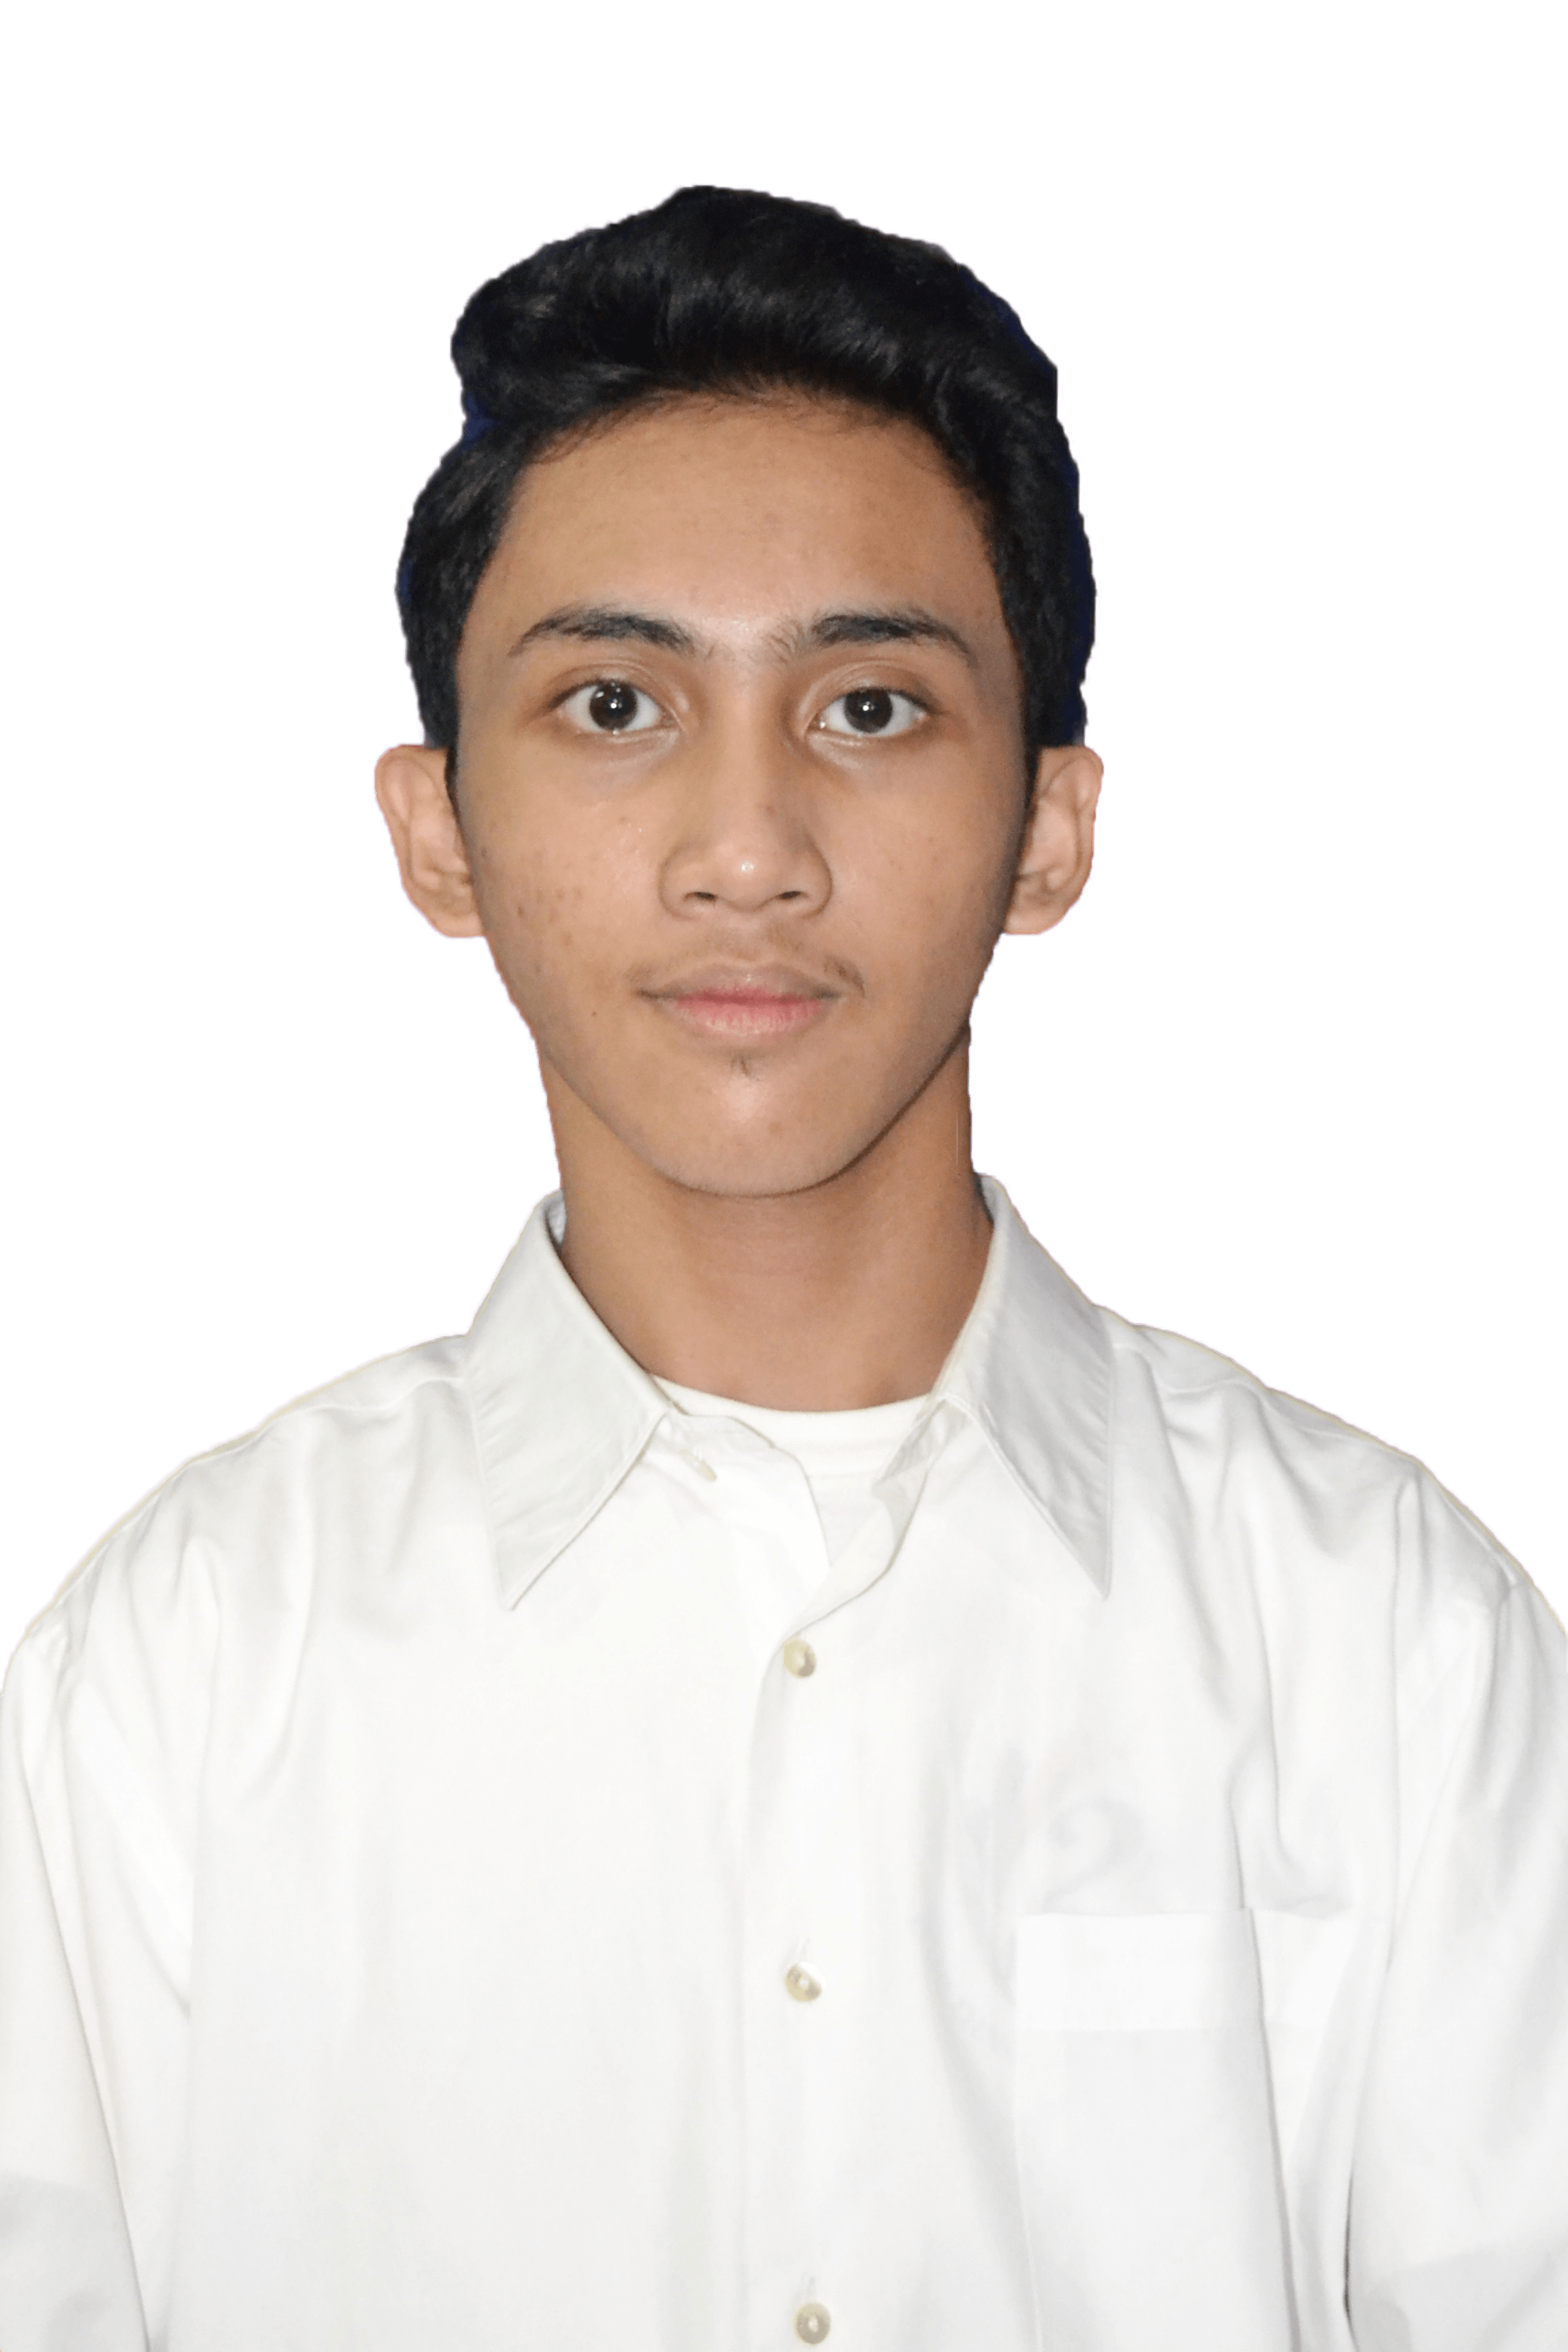
\includegraphics[width=0.3\textwidth]{BiografiPenulis/5024221026_Mahija Ibad Pradipta.png}
	\vspace{-4ex}
\end{wrapfigure}

% Ubah kalimat berikut dengan biografi dari mahasiswa
\name{}, atau yang biasa dikenal sebagai Mahija, lahir di Jakarta Pusat pada 7 Mei 2005. Penulis merupakan anak ketiga dari empat bersaudara yang tinggal dan tumbuh besar di Kota Jakarta. Ketertarikan mendalam penulis di bidang teknologi mengantarkan penulis yang telah menyelesaikan masa sekolah di SMA Negeri 4 Jakarta ke jenjang strata satu di Departemen Teknik Komputer Fakultas Teknologi Elektro dan Informatika Cerdas Institut Teknologi Sepuluh Nopember (ITS) pada tahun 2022.

Penulis merupakan pribadi yang memiliki ketertarikan pada olahraga, ekplorasi alam, maupun menjelajahi topik - topik yang berkaitan dengan bidang teknologi baik software, hardware maupun integrasinya. Ataupun diluar teknologi seperti administrasi, keuangan, dan manajerial. Terbukti dalam masa kuliah, penulis banyak menyelesaikan proyek keperluan tugas mata kuliah yang berkaitan dengan software, hardware, maupun IoT. Selain itu didukung juga dengan rekam jejak organisasi dan kepanitian dari penulis seperti Kepala Divisi Event Multimedia and Game Event (MAGE) X, Kepala Divisi Official Tim Robotika Banyubramanta ITS, Kepala Departemen Kaderisasi HIMATEKKOM ITS 2025/2026. Serta Koordinator Asisten Laboratorium Multimedia dan \emph{Internet Of Things} (IOT). Hingga saat ini penulis masi terus mengembangkan diri baik secara teknis maupun non teknis. 

Pada penelitian tugas akhir ini, penulis memilih mengembangkan drone otonom untuk mendeteksi korban bencana yang berfokus pada integrasi hardware dan software serta penerapan visi komputer. Penulis berharap hasil penelitian ini dapat menjadi kontribusi nyata terhadap pengembangan teknologi pencarian dan penyelamatan di Indonesia. Bagi pembaca yang memiliki kritik, saran, atau pertanyaan mengenai tugas akhir ini dapat menghubungi penulis melalui surel mahijapradipta86@gmail.com.
